% Options for packages loaded elsewhere
\PassOptionsToPackage{unicode}{hyperref}
\PassOptionsToPackage{hyphens}{url}
%
\documentclass[
]{article}
\title{Latency}
\author{Marisangila Alves}
\date{10/26/2021}

\usepackage{amsmath,amssymb}
\usepackage{lmodern}
\usepackage{iftex}
\ifPDFTeX
  \usepackage[T1]{fontenc}
  \usepackage[utf8]{inputenc}
  \usepackage{textcomp} % provide euro and other symbols
\else % if luatex or xetex
  \usepackage{unicode-math}
  \defaultfontfeatures{Scale=MatchLowercase}
  \defaultfontfeatures[\rmfamily]{Ligatures=TeX,Scale=1}
\fi
% Use upquote if available, for straight quotes in verbatim environments
\IfFileExists{upquote.sty}{\usepackage{upquote}}{}
\IfFileExists{microtype.sty}{% use microtype if available
  \usepackage[]{microtype}
  \UseMicrotypeSet[protrusion]{basicmath} % disable protrusion for tt fonts
}{}
\makeatletter
\@ifundefined{KOMAClassName}{% if non-KOMA class
  \IfFileExists{parskip.sty}{%
    \usepackage{parskip}
  }{% else
    \setlength{\parindent}{0pt}
    \setlength{\parskip}{6pt plus 2pt minus 1pt}}
}{% if KOMA class
  \KOMAoptions{parskip=half}}
\makeatother
\usepackage{xcolor}
\IfFileExists{xurl.sty}{\usepackage{xurl}}{} % add URL line breaks if available
\IfFileExists{bookmark.sty}{\usepackage{bookmark}}{\usepackage{hyperref}}
\hypersetup{
  pdftitle={Latency},
  pdfauthor={Marisangila Alves},
  hidelinks,
  pdfcreator={LaTeX via pandoc}}
\urlstyle{same} % disable monospaced font for URLs
\usepackage[margin=1in]{geometry}
\usepackage{color}
\usepackage{fancyvrb}
\newcommand{\VerbBar}{|}
\newcommand{\VERB}{\Verb[commandchars=\\\{\}]}
\DefineVerbatimEnvironment{Highlighting}{Verbatim}{commandchars=\\\{\}}
% Add ',fontsize=\small' for more characters per line
\usepackage{framed}
\definecolor{shadecolor}{RGB}{248,248,248}
\newenvironment{Shaded}{\begin{snugshade}}{\end{snugshade}}
\newcommand{\AlertTok}[1]{\textcolor[rgb]{0.94,0.16,0.16}{#1}}
\newcommand{\AnnotationTok}[1]{\textcolor[rgb]{0.56,0.35,0.01}{\textbf{\textit{#1}}}}
\newcommand{\AttributeTok}[1]{\textcolor[rgb]{0.77,0.63,0.00}{#1}}
\newcommand{\BaseNTok}[1]{\textcolor[rgb]{0.00,0.00,0.81}{#1}}
\newcommand{\BuiltInTok}[1]{#1}
\newcommand{\CharTok}[1]{\textcolor[rgb]{0.31,0.60,0.02}{#1}}
\newcommand{\CommentTok}[1]{\textcolor[rgb]{0.56,0.35,0.01}{\textit{#1}}}
\newcommand{\CommentVarTok}[1]{\textcolor[rgb]{0.56,0.35,0.01}{\textbf{\textit{#1}}}}
\newcommand{\ConstantTok}[1]{\textcolor[rgb]{0.00,0.00,0.00}{#1}}
\newcommand{\ControlFlowTok}[1]{\textcolor[rgb]{0.13,0.29,0.53}{\textbf{#1}}}
\newcommand{\DataTypeTok}[1]{\textcolor[rgb]{0.13,0.29,0.53}{#1}}
\newcommand{\DecValTok}[1]{\textcolor[rgb]{0.00,0.00,0.81}{#1}}
\newcommand{\DocumentationTok}[1]{\textcolor[rgb]{0.56,0.35,0.01}{\textbf{\textit{#1}}}}
\newcommand{\ErrorTok}[1]{\textcolor[rgb]{0.64,0.00,0.00}{\textbf{#1}}}
\newcommand{\ExtensionTok}[1]{#1}
\newcommand{\FloatTok}[1]{\textcolor[rgb]{0.00,0.00,0.81}{#1}}
\newcommand{\FunctionTok}[1]{\textcolor[rgb]{0.00,0.00,0.00}{#1}}
\newcommand{\ImportTok}[1]{#1}
\newcommand{\InformationTok}[1]{\textcolor[rgb]{0.56,0.35,0.01}{\textbf{\textit{#1}}}}
\newcommand{\KeywordTok}[1]{\textcolor[rgb]{0.13,0.29,0.53}{\textbf{#1}}}
\newcommand{\NormalTok}[1]{#1}
\newcommand{\OperatorTok}[1]{\textcolor[rgb]{0.81,0.36,0.00}{\textbf{#1}}}
\newcommand{\OtherTok}[1]{\textcolor[rgb]{0.56,0.35,0.01}{#1}}
\newcommand{\PreprocessorTok}[1]{\textcolor[rgb]{0.56,0.35,0.01}{\textit{#1}}}
\newcommand{\RegionMarkerTok}[1]{#1}
\newcommand{\SpecialCharTok}[1]{\textcolor[rgb]{0.00,0.00,0.00}{#1}}
\newcommand{\SpecialStringTok}[1]{\textcolor[rgb]{0.31,0.60,0.02}{#1}}
\newcommand{\StringTok}[1]{\textcolor[rgb]{0.31,0.60,0.02}{#1}}
\newcommand{\VariableTok}[1]{\textcolor[rgb]{0.00,0.00,0.00}{#1}}
\newcommand{\VerbatimStringTok}[1]{\textcolor[rgb]{0.31,0.60,0.02}{#1}}
\newcommand{\WarningTok}[1]{\textcolor[rgb]{0.56,0.35,0.01}{\textbf{\textit{#1}}}}
\usepackage{graphicx}
\makeatletter
\def\maxwidth{\ifdim\Gin@nat@width>\linewidth\linewidth\else\Gin@nat@width\fi}
\def\maxheight{\ifdim\Gin@nat@height>\textheight\textheight\else\Gin@nat@height\fi}
\makeatother
% Scale images if necessary, so that they will not overflow the page
% margins by default, and it is still possible to overwrite the defaults
% using explicit options in \includegraphics[width, height, ...]{}
\setkeys{Gin}{width=\maxwidth,height=\maxheight,keepaspectratio}
% Set default figure placement to htbp
\makeatletter
\def\fps@figure{htbp}
\makeatother
\setlength{\emergencystretch}{3em} % prevent overfull lines
\providecommand{\tightlist}{%
  \setlength{\itemsep}{0pt}\setlength{\parskip}{0pt}}
\setcounter{secnumdepth}{-\maxdimen} % remove section numbering
\ifLuaTeX
  \usepackage{selnolig}  % disable illegal ligatures
\fi

\begin{document}
\maketitle

\hypertarget{paruxe2metros}{%
\subsubsection{Parâmetros}\label{paruxe2metros}}

\begin{verbatim}
Parâmetros      | Valores
----------------------|----------
alfa zipf             | 0.8 
lambda                | 5
n                     | 100
beta                  | 0.2
BS                    | 32
Cache                 | 100
UE                    | 200
Storage               | MBS: 20GB - SBS: 4GB
Coverage              | MBS 300 SBS 70
RTT inicial           | CS/MBS 0.001s(1ms) MBS/MBS 0.001s(1ms) MBS/SBS 0.001s(1ms) / SBS/UE 0.001s(1ms) / CLOUD/UE 0.01 (10ms)
Tempo da Requisição   | 10 eventos
Mobilidade            | 10m
\end{verbatim}

\hypertarget{informauxe7uxf5es-da-aplicauxe7uxe3o.}{%
\subsubsection{Informações da
Aplicação.}\label{informauxe7uxf5es-da-aplicauxe7uxe3o.}}

\begin{verbatim}
Vazão Mínima |     Tamanho da Cache        | Buffer |
-------------|-----------------------------|--------|
 100 Mbps |      2GB/2000MB             |  48Mb  |
 100 Mbps |      4GB/4000MB             |  48Mb  |
 100 Mbps |      8GB/8000MB             |  48Mb  |
\end{verbatim}

\hypertarget{distribuiuxe7uxe3o-da-latuxeancia}{%
\subsubsection{Distribuição da
Latência}\label{distribuiuxe7uxe3o-da-latuxeancia}}

\hypertarget{distribuiuxe7uxe3o.}{%
\subsubsection{Distribuição.}\label{distribuiuxe7uxe3o.}}

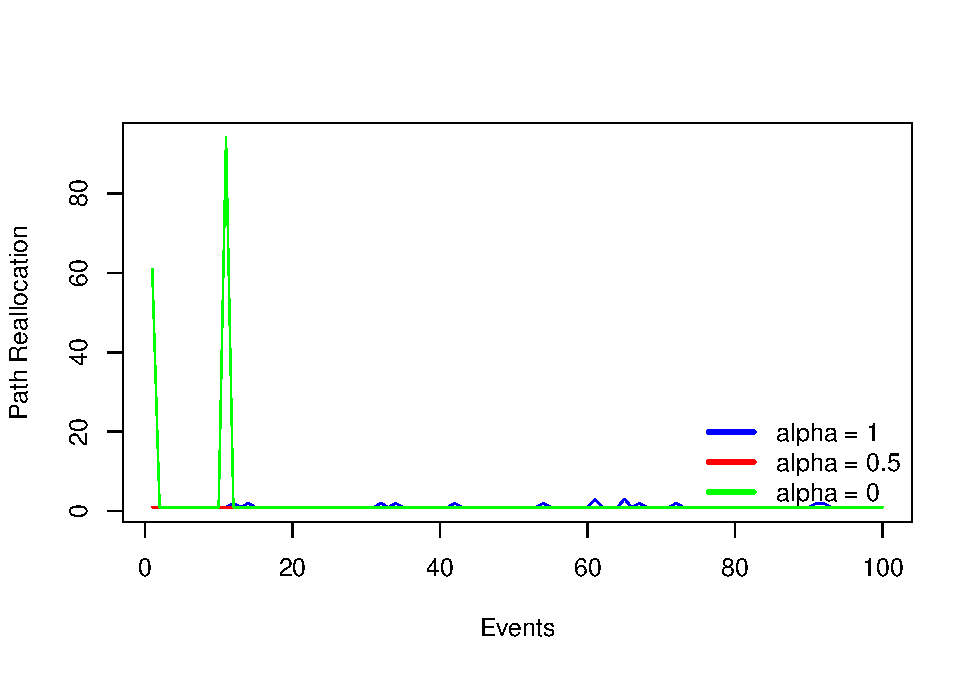
\includegraphics{lantecy_models_files/figure-latex/unnamed-chunk-10-1.pdf}

\begin{verbatim}
## Saving 6.5 x 4.5 in image
\end{verbatim}

\hypertarget{delay-muxe9dio-das-requisiuxe7uxf5es-por-evento.}{%
\subsubsection{Delay Médio das Requisições por
Evento.}\label{delay-muxe9dio-das-requisiuxe7uxf5es-por-evento.}}

\begin{Shaded}
\begin{Highlighting}[]
\ControlFlowTok{for}\NormalTok{(i }\ControlFlowTok{in} \DecValTok{1}\SpecialCharTok{:}\NormalTok{n)\{}
  \ControlFlowTok{if}\NormalTok{(delay\_links\_median\_multi\_hop[i] }\SpecialCharTok{\textgreater{}} \DecValTok{8}\NormalTok{)\{}
    \FunctionTok{print}\NormalTok{(i)}
\NormalTok{  \}}
\NormalTok{\}}
\end{Highlighting}
\end{Shaded}

\begin{verbatim}
## [1] 18
## [1] 51
## [1] 69
## [1] 70
## [1] 71
## [1] 74
## [1] 81
\end{verbatim}

\includegraphics{lantecy_models_files/figure-latex/unnamed-chunk-19-1.pdf}

\begin{verbatim}
## Saving 6.5 x 4.5 in image
\end{verbatim}

\hypertarget{somuxe1torio-delay-das-requisiuxe7uxf5es-por-evento.}{%
\subsubsection{Somátorio Delay das Requisições por
Evento.}\label{somuxe1torio-delay-das-requisiuxe7uxf5es-por-evento.}}

\includegraphics{lantecy_models_files/figure-latex/unnamed-chunk-23-1.pdf}

\begin{verbatim}
## Saving 6.5 x 4.5 in image
\end{verbatim}

\hypertarget{distribuiuxe7uxe3o.-1}{%
\subsubsection{Distribuição.}\label{distribuiuxe7uxe3o.-1}}

\includegraphics{lantecy_models_files/figure-latex/unnamed-chunk-27-1.pdf}

\begin{verbatim}
## Saving 6.5 x 4.5 in image
\end{verbatim}

\hypertarget{regressuxe3o-nuxe3o-linear.}{%
\subsubsection{Regressão Não
Linear.}\label{regressuxe3o-nuxe3o-linear.}}

\includegraphics{lantecy_models_files/figure-latex/unnamed-chunk-29-1.pdf}
\includegraphics{lantecy_models_files/figure-latex/unnamed-chunk-29-2.pdf}
\includegraphics{lantecy_models_files/figure-latex/unnamed-chunk-29-3.pdf}

\hypertarget{histogramas.}{%
\subsubsection{Histogramas.}\label{histogramas.}}

\includegraphics{lantecy_models_files/figure-latex/unnamed-chunk-30-1.pdf}
\includegraphics{lantecy_models_files/figure-latex/unnamed-chunk-30-2.pdf}
\includegraphics{lantecy_models_files/figure-latex/unnamed-chunk-30-3.pdf}

\hypertarget{resumo-one-hop}{%
\subsubsection{Resumo One-hop}\label{resumo-one-hop}}

\begin{verbatim}
##    Min. 1st Qu.  Median    Mean 3rd Qu.    Max. 
##   1.000   1.786  10.000   7.507  10.000  10.000
\end{verbatim}

\begin{verbatim}
##     0%    25%    50%    75%   100% 
##  1.000  1.786 10.000 10.000 10.000
\end{verbatim}

\begin{verbatim}
## 95% 
##  10
\end{verbatim}

\hypertarget{resumo-multi-hop}{%
\subsubsection{Resumo Multi-hop}\label{resumo-multi-hop}}

\begin{verbatim}
##    Min. 1st Qu.  Median    Mean 3rd Qu.    Max. 
##   1.000   1.757  10.000   7.148  10.000  10.000
\end{verbatim}

\begin{verbatim}
##     0%    25%    50%    75%   100% 
##  1.000  1.757 10.000 10.000 10.000
\end{verbatim}

\begin{verbatim}
## 95% 
##  10
\end{verbatim}

\hypertarget{resumo-network-aware}{%
\subsubsection{Resumo Network-aware}\label{resumo-network-aware}}

\begin{verbatim}
##    Min. 1st Qu.  Median    Mean 3rd Qu.    Max. 
##   1.000   1.414   3.029   3.328   5.029  19.000
\end{verbatim}

\begin{verbatim}
##     0%    25%    50%    75%   100% 
##  1.000  1.414  3.029  5.029 19.000
\end{verbatim}

\begin{verbatim}
## 95% 
##   7
\end{verbatim}

\hypertarget{teste-t-nuxe3o-pareado.}{%
\subsubsection{Teste T não pareado.}\label{teste-t-nuxe3o-pareado.}}

\begin{verbatim}
## [1] "Há diferença significativa."
\end{verbatim}

\begin{verbatim}
## 
##  Welch Two Sample t-test
## 
## data:  delay_one_hop$Delay and delay_multi_hop$Delay
## t = 4.1444, df = 8421.7, p-value = 3.441e-05
## alternative hypothesis: true difference in means is not equal to 0
## 95 percent confidence interval:
##  0.1894900 0.5296208
## sample estimates:
## mean of x mean of y 
##  7.507386  7.147830
\end{verbatim}

\begin{verbatim}
## [1] "Há diferença significativa."
\end{verbatim}

\begin{verbatim}
## 
##  Welch Two Sample t-test
## 
## data:  delay_one_hop$Delay and delay_network_aware$Delay
## t = 61.328, df = 6324.8, p-value < 2.2e-16
## alternative hypothesis: true difference in means is not equal to 0
## 95 percent confidence interval:
##  4.045416 4.312577
## sample estimates:
## mean of x mean of y 
##  7.507386  3.328389
\end{verbatim}

\begin{verbatim}
## [1] "Há diferença significativa."
\end{verbatim}

\begin{verbatim}
## 
##  Welch Two Sample t-test
## 
## data:  delay_multi_hop$Delay and delay_network_aware$Delay
## t = 54.848, df = 6226.4, p-value < 2.2e-16
## alternative hypothesis: true difference in means is not equal to 0
## 95 percent confidence interval:
##  3.682930 3.955953
## sample estimates:
## mean of x mean of y 
##  7.147830  3.328389
\end{verbatim}

\end{document}
